\chapter{Basic operations} \label{chap:basicop}


    \section{Introduction} 
This chapter introduces some of the most basic ingredients that support the programming.
Data types, data structures, maths operators or flow structures are some of the most basic concepts needed to code in any programming language. 
But first let's put them in context. 

An algorithm in mathematics is a finite sequence of unambiguous instructions to solve a specific problem. 
Notice that this definition involves that the algorithm ends in a finite number of steps, 
the sequence of instructions that yields the output are numbered and followed in their numerical order and
inputs, instructions and outputs must be properly identified. 

The problem can be seen as a function between a bunch of inputs and their associated outputs.
If we particularize it on a specific set of inputs we have an instance of that problem, 
then, we need an algorithm to solve the instance.
The theory of computation gives the basis for the automatic processing of the algorithm, it needs from a 
problem to solve, an algorithm that solves it and a machine to compute it 
and gives answers for example to how efficiently the problem is going to be solved. 

To take advantage of the use of machines that compute the algorithm automatically we use programs.
The program or code is the translation of the algorithm expressed in a mathematical language to a language understood by 
the machine, the programming language. 

In conclusion, the algorithm breaks down a complex problem into simpler instructions 
and the program translates those steps so the machine can understand them. 
To translate these instructions each programming language offers a bunch of building blocks.
Most programming languages have the same components as building blocks:
\begin{itemize}[noitemsep]
    \item \textbf{Statements and Expressions:} Statements are all lines of code that instructs the compiler to perform a task.
    There are several types of statements like assignments, procedures calls, input/output statements or flow control structures. 
    It is usually distinguished between statements and expressions. 
    The former are executed with no value as a result, only an instruction, 
    and the latter are evaluated to determine a resulting value.
    
    \item \textbf{Variables and data structures:} a variable is a tag that identifies a piece of data, 
    it's a reference to the memory space holding the data but not the data itself. 
    Actually, this data attached may change during the execution of the program. 
    Some data types commonly found are integer, real, complex, logical or character.
    In contrast, \textbf{constants} may also have a name but their attached data don't change during the execution.
    Data structures are also used to store, organize and process data, 
    now arranged in a specific way so that it can be treated efficiently. 
    Some common data structures are arrays, sets, lists, tuples, trees, graphs, etc.
    
    \item \textbf{Operators:} These are symbols that tells the compiler to perform operations of different kind in order to produce a result.
    There are arithmetic (addition, subtraction, multiplication, division, etc.), 
    relational (greater than, less than, equal to, different to, etc.) and 
    logical operators (AND, OR, NOT). 
    Sometimes the assignment operator (\texttt{=}) is also included in this classification, 
    however, it has a different nature compared to the others. 
    
    \item \textbf{Control flow structures:} These are the structures that, by means of keywords, allow to control the flow of data along the program. 
    Essentially they allow the program to take decisions and execute instructions in a certain way depending on those decisions. 
    The most basic control structures are the loops and the conditionals. 
    
    \item \textbf{Comments:} This is a line of code that is not read or executed by the compiler and 
    that is intended to help the programmer understand the code.
    
    %\item \textbf{Procedures, Objects, etc:}
\end{itemize}

Some other keywords and characters are usually reserved by the programming language in order to perform different tasks. 
These keywords depend on each language and can be used for example to 
group numbers (parenthesis), 
delimit characters (\texttt{''}), 
indicate classes or methods,
break lines of code, etc.

Finally, there is a different kind of statement that is not part of the programming language itself 
but also instructs the compiler to perform tasks; the compiler directives. 
These statements cause the compiler to take a specific action during compilation and may vary from compiler to compiler.


%MORE:
%Input: getting data and commands into the computer
%Output: getting your results out of the computer

%Libro FORTRAN: Programación Multicapa

%Most important basic elements for programming languages are:
%Programming Environment
%Keywords
%Input and Output Operations

%Functions
%A function is a statement that returns a value. For example, the function InputBox() returns the value of its dialog text field.
%Objects
%An object is a program “building block” entity. It can be visible, like a Button control, or invisible like a Timer control.
%Properties
%A property is a characteristic of an object. For example, the property Btn.Text is the Text property of the Btn object.
%Methods
%A method is an action that an object can perform. For example, the method Btn.Click() is the Click method of the Btn object.



%The assignment statement \texttt{v = 3*5 + 2} becomes the bottleneck of programming languages in the sense that a program is mainly concerned 
%with the flow of assignments of single variables (imitating single words). 
%By executing assignments many times, maybe altering subscripts (imitating memory addresses), 
%the program ends up with the result stored in a variable (imitating the storage in memory). 
%Furthermore, this assignment statement splits the programming languages into two worlds: 
%a world of expressions with strong algebraic properties (\texttt{3*5 + 2}) and a world of statements with few mathematical properties (\texttt{v =}).




    \section{Data types}
    
Several objects are used to build the different branches of mathematics; numbers, operations, functions, sets, vectors, matrices, tensors and a large etcetera. 
Let's review here the formal definition of some objects that later are represented in programming by means of the data types. 

The set of integers $\mathbb{Z}$ includes the number zero (0), the natural numbers ($\mathbb{N} = \{ 1,2,3,... \}$) and their additive inverses, the negative numbers ($\{ -1,-2,-3,... \}$).
The set of real numbers ($\mathbb{R}$) includes any number identified with a point on the real number line.
This set includes both the set of rational numbers ($\mathbb{Q}$) and the set of irrational numbers.
Finally, the complex numbers ($\mathbb{C}$) extends the real numbers using the imaginary unit, an element satisfying the equation $i^2 = -1$.
This equation does not have solution among the real numbers and, 
once introduced the imaginary unit, every complex number can be expressed as $a+bi$ where $a,b\in\mathbb{R}$. 

In the context of the elementary algebra, some operations are defined for the elements of each of these sets.
Furthermore, the operations together with the sets accomplish with a bunch of algebraic properties that give them 
a ring structure to the integers 
or a field structure in the case of reals or complex numbers. 

In a different context, the Boolean algebra, the values of the variables are the truth values: true and false instead of numbers.
Also, the basic operations are conjunction (and), disjunction (or) and negation (not) instead of binary operations like addition and multiplication.

In a similar way, each constant, variable, array or function in a programming language has an intrinsic data type associated. 
This type decides, among other things, the allowed values that the entity can have and the set of operations that can be performed with them.
For example, the set of integers in mathematics are represented in a programming language through \texttt{integer} data type. 
Then, a value $x\in \mathbb{Z}$ will be stored in an \texttt{integer} variable and operations like addition, multiplication or exponentiation are allowed. 

The data typing in a programming language is explicit when the programmer needs to decide and declare the type for each variable or implicit when the language assumes it. 
Furthermore, while some programming languages allow the use of some data types as if they were a different type (weak typing) others does not (strong typing). 
Python is mainly an implicit typing language since we can assign a value to a variable without declaring type, i.e. \texttt{a = 3} will automatically treat \texttt{a} as an integer. 
Fortran, on the contrary, is a explicit typing language because all variables must be previously declared with a specific type, i.e. \texttt{real :: x = 5.6}.



        \newpage
        \subsection*{Fortran code}

Fortran provides five intrinsic data types. 
Derived data types can be created either from intrinsic data types or from other derived types previously defined.
The five intrinsic types are:
\begin{itemize}
    \item Numeric nature: \texttt{integer}, \texttt{real}, \texttt{complex}. 
    \item Boolean nature: \texttt{logical}.
    \item Text nature: \texttt{character}.
\end{itemize}
The numeric types behave like the mathematical abstractions of these sets, 
roughly speaking: $n\in \mathbb{Z}$ is stored in an \texttt{integer}, 
$x\in \mathbb{R}$ is stored in an \texttt{real} and 
$z\in \mathbb{C}$ is stored in an \texttt{complex} variable.
Many nuances to the equivalence between the programming concept and the mathematical abstraction for integers and reals are treated in the Part \ref{PartII} of this book. 
The \texttt{logical} type gets the two possible values of the Boolean algebra; \texttt{True} and \texttt{False}. 
Finally, the \texttt{character} type can store strings with ASCII characters which includes alphanumeric, symbols and sign characters.   

Since Fortran is an explicit typing language, before using any variable, all must be previously declared with a specific type.
The following program shows an example of the declaration and initialization of the five data types we can find. 
\vspace{0.5cm}
\lstfor
\renewcommand{\home}{./Fortran/sources/Foundations/Basic operations} 
\listings{\home/Basic_operations.f90}{subroutine Data_types}
{end subroutine}{Basic_operations.f90}



        \newpage 
        \subsection*{Python code}

The same five data types are built-in in Python but with a different name: 
\begin{itemize}
    \item Numeric nature: \texttt{int}, \texttt{float}, \texttt{complex}. 
    \item Boolean nature: \texttt{bool}.
    \item Text nature: \texttt{str}.
\end{itemize}

Since Python is an implicit typing language don't declare the type of any variable and just initialize it.
The following program shows an example of the initialization of the five data types we can find. 
\vspace{0.5cm} 
\renewcommand{\home}{./Python/sources/Foundations/Data_type} 
\lstpython
\listings{\home/data_type.py}{def data_types}
{string}{data_type.py} 




    \newpage
    \section{Data structures} 

Numbers and truth values are not the only objects needed to build the different branches of mathematics.
Also sets, vectors, tuples, matrices, tensors or sequences are used in the context of algebra, calculus or set theory.
Let's review now the formal definition of the objects that later are represented in programming by arrays, sets, tuples and lists. 

%set
A set, with the definition given by Georg Cantor within the set theory, 
is a gathering together into a whole of definite, distinct objects of our perception or our thought, 
which are called elements of the set.
The elements of a set can be any mathematical objects: numbers, points in space, geometrical shapes, variables or other sets.
However, every element of the set must be different from the others.

Tuples and sequences are also collections of mathematical objects.
However, a sequence is an enumerated collection, where repetitions are allowed and order matters.
Unlike sets, since the elements follow an order, the elements can be repeated in different positions of the sequence.
A sequence can also be interpreted as a function from $\mathbb{N}$ (denoting the position within the sequence) to the elements.
The length of the sequence is its number of elements and could be any finite value or infinite. 
A tuples is a finite sequence, which means, a finite ordered lists of elements. 
It is usually used the notation $n-$tuple for a list of $n$ elements, where $n$ is a non-negative integer.

%vectors
The concept of vector in mathematics has different formal definitions depending on the context.
Historically the term vector was used for geometric vectors, objects that has magnitude and direction.
However, a vector can be nowadays seen as a tuple or, in pure mathematics, as any element of a vector space. 

Indeed, vectors considered as tuples of elements in a field $\mathbb{F}$, together with the common addition of vectors and the multiplication by an scalar in the field $\mathbb{F}$, build a vector space. 
It is usually used $\mathbb{F}^{n}$ to denote the set of all $n-$tuples with entries in the field $\mathbb{F}$, that could be for example $\mathbb{R}$ or $\mathbb{C}$. 
Hence, $\mathbb{R}^{2}$ or $\mathbb{R}^{3}$ are 2-tuples and 3-tuples of reals and conform vector spaces with all its linear combinations.
Notice that a vector can be represented by a one-dimensional arrangement of $n$ elements with respect to a given basis.

A matrix is a rectangular arrangement of numbers (or other mathematical objects) distributed in rows and columns.
Matrices over a field $\mathbb{F}$ are those where all its \textit{elements} or \textit{entries} are elements of the field $\mathbb{F}$.
If $\mathbb{F}$ is $\mathbb{R}$ or $\mathbb{C}$ it conforms real matrices or complex matrices respectively.
It is usually used $\mathbb{F}^{n\times m}$ or  ${ \cal{M}}^{n \times m} (\mathbb{F})$ to denote the set of $n\times m$ matrices with entries in the field $\mathbb{F}$. 
This set, together with the common addition of matrices and the multiplication by numbers (scalars) in the field $\mathbb{F}$ have the structure of vector space. 
Hence, the matrices are also vectors inherited from the vector space structure they present.

%Tensors are NOT the generalization of scalars, vectors and matrices (no indices, one index, two indices) to an arbitrary number of indices. 
The concept of tensor, like the concept of vector, also has different approaches. 
Avoiding the formal definition let's consider here that a tensor can be represented as a potentially multidimensional array.
The elements in this multidimensional array are called its scalar components and are denoted by indices denoting their position in the array.

The standard notation for all these objects are as indicated below:
\begin{itemize}
    \item Sets are usually indicated by listing its elements between curly brackets $\{\}$ separated by commas (roster notation): $\{\textrm{car, boat, plane}\}$
    \item Sequences and tuples are usually written between parenthesis $()$ or less often using square brackets $[]$ or angle brackets $\langle \rangle$: $(1,3,5,7,...)$
    \item In a similar way vectors are usually enclosed in either parentheses $()$ or angle brackets $\langle \rangle$: $(1,2,3,4,5)$ or $\langle1,2,3,4,5 \rangle$
    \item Matrices are commonly written with square brackets or parentheses:
    
    $
    \begin{bmatrix}
        1 & 2 & 3 \\
        4 & 5 & 6
    \end{bmatrix} 
    $ or $
    \begin{pmatrix}
        1 & 2 & 3\\
        4 & 5 & 6
    \end{pmatrix}   
    $
    \item A tensor is usually denoted by a symbolic name followed by a collection of subscripts where the number of subscripts attached defines the rank of the tensor.
    For example $\alpha_{ijkl}$ is a rank 4 tensor.
\end{itemize}

In a programming language all these objects are represented by different data structures.
Fortran for example does not include tuples, sets or sequences, but vectors, matrices and tensors are represented by arrays. 
On the contrary, Python has built-in the structures of sets and tuples among others and arrays are available in the library \texttt{NumPy}.  

With the Fortran examples below the following concepts are covered:
\begin{enumerate}[noitemsep]
    \item Declaring arrays: type, rank and dimension.
    \item Initialize arrays: constructors. 
    \item Iterators for arrays: sectors or slices. 
\end{enumerate}

Also, with the Python examples, the following concepts are treated:
\begin{enumerate}[noitemsep]
    \item Constructors, iterators and slices for NumPy arrays.
    \item Using sets, lists, tuples and dictionaries: constructors.
    \item Iterators for data structures.
\end{enumerate}





        \newpage
        \subsection*{Fortran code}
%Declaration
Consider the following vectors $V, W \in \mathbb{R}^N$, $X\in \mathbb{R}^6$, $Y\in \mathbb{R}^3$ and matrix $A \in { \cal{M}}^{N \times N} (\mathbb{R})$ 
with $N=10$ and let's declare them using Fortran arrays. 
$$
V = \left( v_i =\frac{1}{i^2} \right)^T, \quad W = \left( w_i = \frac{(-1)^{i+1}}{2i+1} \right)^T \;\; i = 1 \ldots  N,  \quad Y = \left(A_{i j}\right)_{\substack{i = 2 \\  3\leq j\leq 5}}^T
$$
$$
A = \left[ a_{ij} = \left( \frac{i}{N} \right)^{j-1}, \ \ i = 1 \ldots  N, \ \ j = 1 \ldots  N \right], \quad X = ( 1.3, 2.4, 3, 4.5, 5.3, 7 )^T
$$
An array, either representing a vector, a matrix or a tensor, is properly \textbf{declared} when it has 
type, rank and dimension (or extent) (see Figure \ref{fig:arrays}). 
The data type has already been treated before, in these examples we are using \texttt{real}. 
The rank; the number of dimensions in the array, is 1 for column vectors, 2 for matrices and can be higher for higher dimension tensors.
The extent of each particular dimension is its length; the number of elements in that dimension.
\begin{IN}
Notice that, in Fortran, the \textbf{bounds of a dimension} may start with the index we prefer. 
By default it stars with index \texttt{1} but it can start in \texttt{0} or whatever index we want. 
For example the matrix \texttt{B(-2:4,0:1)} starts in \texttt{-2} and ends in \texttt{4} (also included) for the first dimension and 
\texttt{0} and \texttt{1} (also included) for the second dimension. 
\end{IN}
\vspace{0.5cm}
\lstfor
\renewcommand{\home}{./Fortran/sources/Foundations/Basic operations} 
\listings{\home/Basic_operations.f90}{subroutine Data_structures}
{4,0}{Basic_operations.f90}




%Initialization
Once declared, the \textbf{initialization} of the arrays is performed with constructors. 
Three ways are commonly used to manually construct an array: 
\vspace{-0.5cm}
\begin{enumerate}[noitemsep]
    \item \textbf{By a list of values:} \texttt{ [ list ] } where 'list' is a list of values of the same array type separated by commas. 
    For example the vector \texttt{X} in the code. 
    \item \textbf{Using an array expression:} \texttt{Y = [ A(2, 3:5) ]} stores the list of values in the second row of \texttt{A} from columns \texttt{3} to \texttt{5}.
    \item \textbf{Using an implicit loop:} a list of elements is computed from a loop. For example vectors \texttt{V}, \texttt{W} or matrix \texttt{A} in the code.
\end{enumerate}
In the case of Fortran the constructors are only used for rank-one arrays so 
functions like \texttt{reshape} are needed for higher ranks. 
For example the matrix \texttt{A} in the code is initialized using the \texttt{reshape} function.     
\vspace{0.2cm}
\lstfor
\renewcommand{\home}{./Fortran/sources/Foundations/Basic operations} 
\listings{\home/Basic_operations.f90}{1./i}
{2, 3}{Basic_operations.f90}    
    
   
  
    
%sectors, iterators... 
In general, Fortran allows only one kind of \textbf{iterator} for arrays; 
an index in the dimension whether it loops with an implicit or explicit loop.   
This is intimately related to the \textbf{slicing} of an array: the initialization of \texttt{Y} in the example above use an slice of \texttt{A}.
This can also be extended to a whole dimension of an array using the colon symbol, \texttt{C(:,2)} (see the example below and Figure \ref{fig:arrays}). 
Furthermore, alternate values can be selected by specifying a lower bound, an upper bound and the jump between values 
(see the example below and Figure \ref{fig:arrays}), \texttt{B(-2:4:3,:)} being the value \texttt{3} the jump between rows.
Notice that, since Fortran is a column major order language, functions like \texttt{reshape} and slicing treats the data by columns. 
\vspace{0.2cm}
\lstfor
\renewcommand{\home}{./Fortran/sources/Foundations/Basic operations} 
\listings{\home/Basic_operations.f90}{!Slices}
{end subroutine}{Basic_operations.f90} 

\begin{figure}
    \begin{subfigure}[b]{0.5\textwidth}
        \centering
        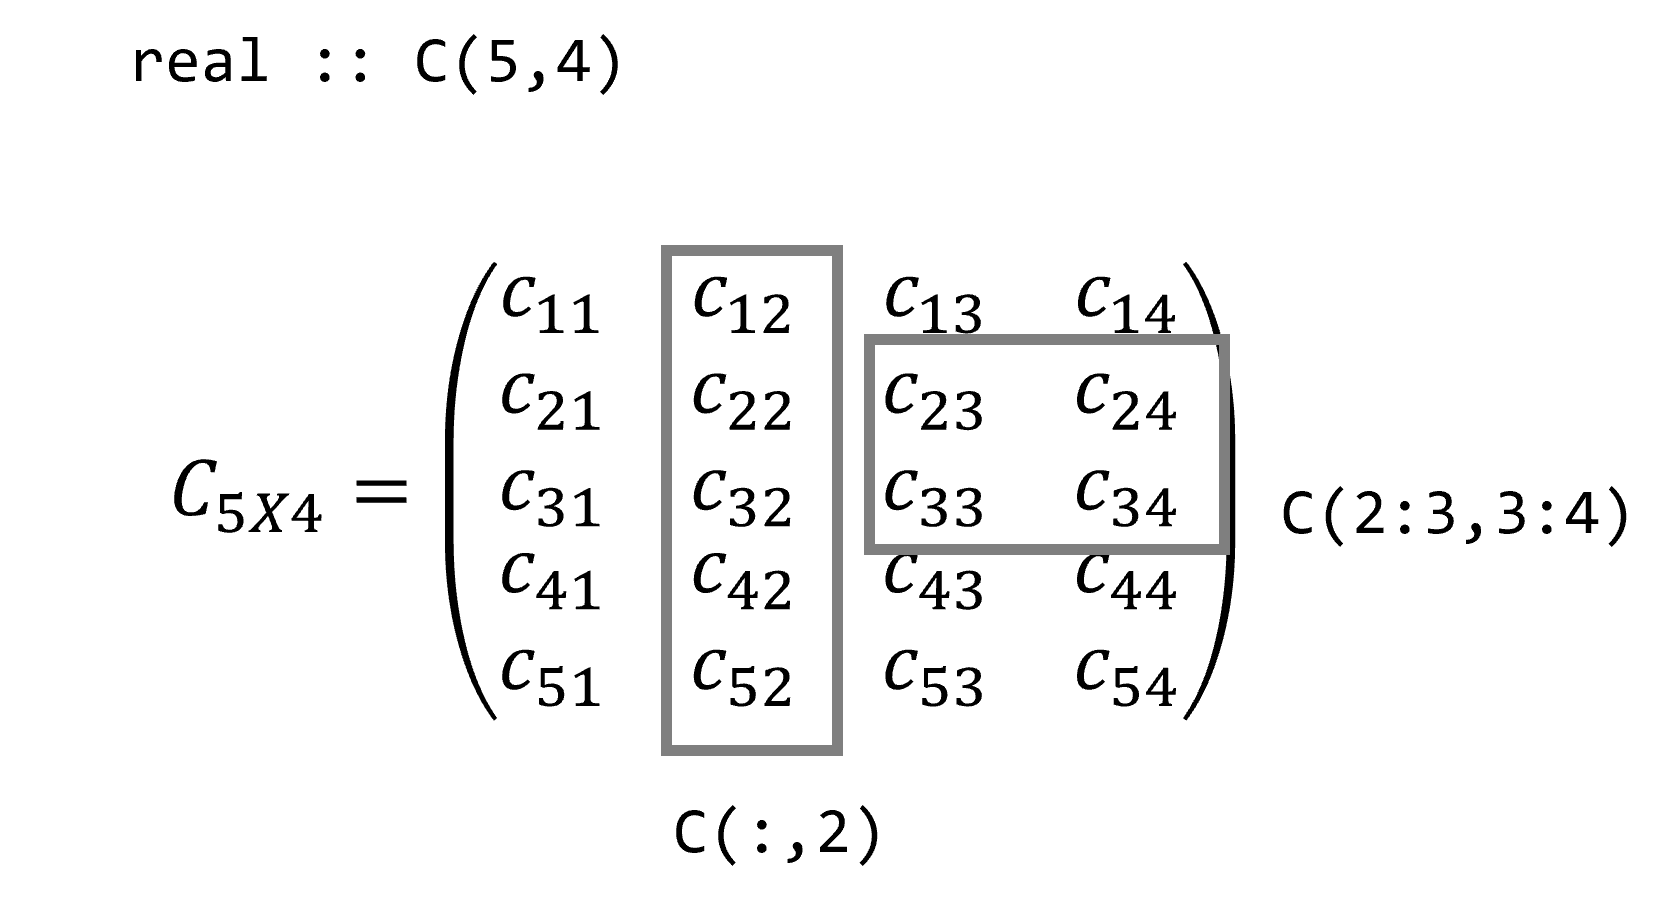
\includegraphics[width = \textwidth]{./doc/Figures/Array1.png}  \\
        \begin{center}
            Rank = 2 \\
            Extent = (5,4) \\
            Size = 20 \\
            Bounds = (1:5, 1:4) \\
            %Shape = (5, 4)
        \end{center}
    \end{subfigure}
    \hspace{\fill}
    \begin{subfigure}[b]{0.5\textwidth}
        \centering
        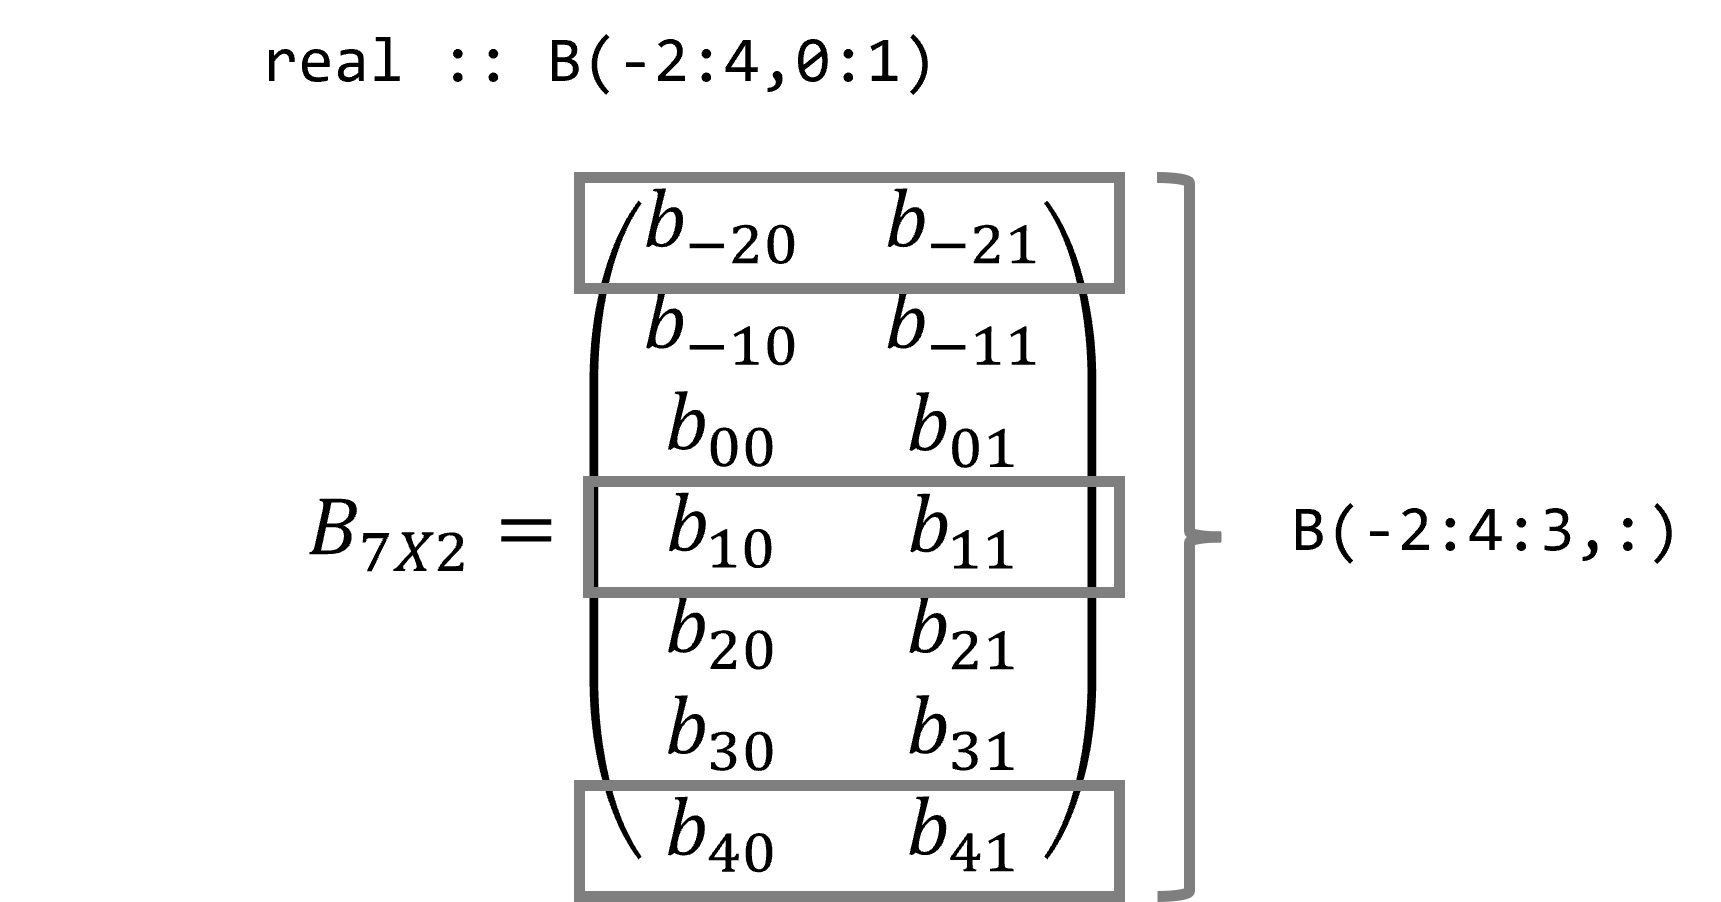
\includegraphics[width = \textwidth]{./doc/Figures/Array3.png}  \\
        \begin{center}
            Rank = 2 \\
            Extent = (7,2) \\
            Size = 14 \\
            Bounds = (-2:4, 0:1) \\
            %Shape = (7, 2)
        \end{center}
    \end{subfigure}
    \caption{Example arrays with their main properties.}   \label{fig:arrays}
\end{figure}







        \newpage 
        \subsection*{Python code}
Let's see the same examples defined above using \texttt{NumPy} arrays and 
let's include now a matrix $Z \in { \cal{M}}^{2 \times 3} (\mathbb{R})$. 
Notice that now they do not need to be explicitly declared, 
Python automatically does it. 
$$
Z =     
\begin{bmatrix}
    1.1 & 2.2 & 3.3\\
    4 & 5.6 & 6.2
\end{bmatrix} 
$$

%Initialization
The \textbf{initialization} of the arrays is performed using the \texttt{array()} function as constructor. 
Three ways are commonly used to manually construct an array: 
\begin{enumerate}[noitemsep]
    \item \textbf{By a list of values:} \texttt{ [ list ] } or \texttt{ [ [ list ], [ list ] ] } where \texttt{list} is a list of values of the same array type separated by commas. 
    For example the vector \texttt{X} or the matrix \texttt{Z}.
    Notice that Python allows manual constructors for higher than rank-one arrays.
    \item \textbf{Using an array expression:} \texttt{Y = A(1, 2:5)} stores the list of values in the second row of \texttt{A} from columns \texttt{3} to \texttt{5}.
    Notice that Python not only starts in \texttt{0} all the indices so \texttt{1} means the second column, 
    but also an slice like \texttt{2:5} ends in \texttt{4} so the slice takes columns \texttt{3} to \texttt{5}. 
    \item \textbf{Using an implicit loop:} a list of elements is computed from a loop. For example vectors \texttt{V}, \texttt{W} or matrix \texttt{A} in the code.
\end{enumerate}
\vspace{0.5cm} 
\lstpython
\renewcommand{\home}{./Python/sources/Foundations/data_type} 
\listingsp{\home/data_type.py}{def arrays}{by rows}{data_type.py}

%sectors, iterators...    
These arrays can be \textbf{iterated} using an index in each dimension and 
\textbf{slicing} is also allowed.
Notice here that NumPy arrays, contrary to Fortran, are row-major order. 
This means that arrays store the data by rows and 
then \texttt{C[1:3 ,2:4] = [ [1.,2.], [3.,4.] ]} will be assigned by rows. 

Similarly to Fortran, the colon symbol iterates in a whole dimension (see \texttt{C[:,1]} in the example above) and 
alternate values can be selected by specifying lower and upper bound and the jump between values.
However, the example \texttt{B(-2:4:3,:)} made with Fortran can not be copied because:
\begin{IN}
In Python, the \textbf{bounds of a dimension} always start with the index \texttt{0} and
the stop value of the slices is never reached. 
\end{IN}









\vspace{0.5cm}
Python has built-in other data structures which are used to store collections of data.
Their elements can be of any type, for example a list can contain strings together with integers and also other lists nested. 
This applies for all the following structures:
\vspace{-.5cm}
\begin{itemize}[noitemsep]    
    \item Set nature: \texttt{set}, \texttt{frozenset}.
    \item Sequence nature: \texttt{list}, \texttt{tuple}.
    \item Mapping nature: \texttt{dict}.
\end{itemize}
\vspace{-.5cm}

%--------------------------------------------------------------------------
A \texttt{set} in Python takes the same meaning as the mathematical object: a collection of any type of data that 
i) is unordered and 
ii) do not allow duplicate values. 
In a set, all that matters is whether each element is in it or not, so the ordering of the elements is irrelevant.
Furthermore, two equal elements, since they are not ordered, could not be distinguished between them. 
A \texttt{frozenset} is an unchangeable set, once created, its content can not be modified. 


%--------------------------------------------------------------------------
%MATEMATICAS:
%List/Sequence: enumerated collection of objects in which repetitions are allowed and order matters. USUALLY INFINITE
%Tuple: enumerated collection of objects in which repetitions are allowed and order matters. ALWAYS FINITE

%PROGRAMMING PYTHON:
%List/Sequence: enumerated collection of objects in which repetitions are allowed and order matters. ONLY FINITE IS POSSIBLE
%Tuple: Same as list but it can not change (programming concept not related to maths)
A \texttt{list} extracts its meaning from the concept of sequence in mathematics,
however, in programming lists can not be infinite.
Hence, a list is characterised by being 
i) ordered: the position within the list is kept, 
ii) allow duplicates: items can appear more than one time in the list and  
iii) changeable: change, add, and remove items are allowed.
In a list, the difference between any two elements comes with the index within the list.
Notice that lists are not arrays or viceversa, in the sense that they come from completely different mathematical concepts. 

A \texttt{tuple} also takes the mathematical definition of tuple (a finite sequence). 
Since both tuples and lists are finite in the computer, the only difference between them are the changeability.
Hence, a tuple is characterised by being 
i) ordered: the position within the tuple is kept, 
ii) allow duplicates: items can appear more than one time in the tuple and  
iii) unchangeable: once created, it can not be modified.
For tuples, Python allocates the required memory once and not reallocates it. 
This becomes a more memory efficient strategy to follow when the data is going to be immutable.



%--------------------------------------------------------------------------
A dictionary (\texttt{dict}) is similar to a list.
It is ordered, changeable and can store any type of data (even other dictionaries nested).
However, unlike lists, the values are stored in pairs: \texttt{key:value} and do not allow the same key for two elements.








\newpage
Let's now take a look at some examples of use cases of these structures. 
Notice that they do not need to be explicitly declared, 
Python automatically does it. 
The following notation is used to manually construct these structures: 
\vspace{-0.5cm}
\begin{itemize}[noitemsep]
    \item \textbf{Set:} Following the roster notation, it is defined by listing its elements between curly brackets and separated by commas.
    \newline Notice that \texttt{ \{``car'', 5, 6.7, 1 + 1j\} } and \texttt{\{5, 1 + 1j, 6.7, ``car'', 5\}} 
    are the same set since repetition and order change do not modify it.
    \item \textbf{List:} Written using square brackets \texttt{[]} with comma-separated values.
    \item \textbf{Tuple:} Written using parenthesis \texttt{()} with comma-separated values. 
    \item \textbf{Dictionary:} It has its list of elements separated by commas, 
    enclosed in curly brackets (\texttt{\{\}}) and 
    using a colon (\texttt{:}) to separate each pair. 
\end{itemize}
%\vspace{0.3cm} 
\lstpython
\renewcommand{\home}{./Python/sources/Foundations/data_type} 
\listingsp{\home/data_type.py}{def data_structures}{returns StopIteration}{data_type.py}




\newpage
Sets, lists, tuples and dictionaries are iterable structures since they all contains a countable number of elements.
Every iterable object can use the \texttt{iter()} method to create an iterator from the data structure.
Also, the \texttt{next()} method is used to jump to the next element in the iterator (\texttt{ite} is created and iterated in the code above).

However, a more straightforward way involves using loops to iterate through the iterable object.
Two main strategies can be followed: 
\begin{enumerate}
    \item \textbf{Iterating in the elements of the structure.} 
    In the code above the set \texttt{S} and the dictionary \texttt{D} are iterated in their elements
    by means of \texttt{s} and \texttt{k} respectively. 
    All iterable structures are iterable in their elements.  
    \item \textbf{Iterating in the index.}
    In the code above both the list and the tuple are iterated in their index \texttt{i} by means of the \texttt{range()} function.
    While lists and tuples are easily iterable on their indices, 
    sets are not subscriptable (they do not have order) and 
    dictionaries need keys as subscripts and not indices. 
\end{enumerate} 

Notice that \texttt{range(start, stop, step)}, with \texttt{start} and \texttt{step} optional arguments, returns a sequence of numbers between the given range.
When only \texttt{stop} is specified (see examples) the iterator starts in \texttt{0} and do not include the stop number itself.
All the arguments of \texttt{range()} are integers, hence, the function \texttt{len()} is used to find the length of the structure to be iterated. 




 

 


%future?
%\texttt{ (/ list /) } is not used as constructor.

%enumerate en Python futuro?

%For sets with many elements, especially those following an implicit pattern,
%the list of members can be abbreviated using an ellipsis ``...''.
%For instance, the set of the first thousand positive integers 
%may be specified in roster notation as
%\begin{verbatim}
%    { 1, 2, 3, ..., 1000 }.
%\end{verbatim}







\newpage
    \section{Maths operators}
    
    
Arithmetic operator 
Comparison operator 
Logical operator 
Membership operator 



In a set the data can be modified through built-in methods so for example mathematical set operations like union, intersection or difference can be performed.



When we want to use all these collections of data, since they are treated as \textit{iterable} objects, we can use a \texttt{for} loop to iterate through them. 
If \texttt{V} is a list, tuple, dictionary or set, we can move throughout all the elements using:
\begin{verbatim}
    for v in V:
\end{verbatim}
So \texttt{v} takes, sequentially, all the values stored in \texttt{V}. 
Notice that, if \texttt{V} is a set, the elements won't follow any specific order. 
Let's execute for example:
\begin{verbatim}
    S = {7,2,"car",78.2,"boat",4.5}
    for x in S:
    print(x)
\end{verbatim}
resulting in:
\begin{verbatim}
    2
    4.5
    7
    boat
    78.2
    car
\end{verbatim}
Use the following expression to iterate using an index throughout the whole length of the collection:
\begin{verbatim}
    for i in range(len(V)): 
\end{verbatim}
or extract both the index and the value of the element using:
\begin{verbatim}
    for i, v in enumerate(V):
\end{verbatim}











    \section{Assignment operators}






    \section{Flow structures}

if 
where 
iterators: list, tuples, arrays, sets, dictionaries (key, value)



for k in D   dictionary iterates in key 
for k in D.keys()   dictionary iterates in keys
for v in D.values()   dictionary iterates in values


\newpage 
    \section{Roots of a second degree equation} 
In this section, a program to obtain the roots of a second order equation is presented:  
$$
a x^2 + b x + c = 0, \qquad \forall \ a, b, c \in \mathbb{R}.
$$
The fundamental theorem of algebra states that every  Nth order polynomial has N complex roots. 
If the coefficients are real, then the roots are complex conjugate.
Dividing the above equation by $ a $ an looking for a perfect square, 
the following equation is obtained: 
$$
\left( x + \frac{b}{2a} \right)^2 - \frac{b^2 }{ 4 a^2} + \frac{c}{a} = 0. 
$$
Solving the unknown $x$, the well known formula for the roots is obtained: 
\begin{equation}
 x_{1,2} = \frac{ - b \pm \sqrt{ b^2 - 4 a c }  }{ 2 a  }  
 \label{x12}
\end{equation} 
If the discriminant $ d = b^2 - 4 a c $ is less than zero, roots become complex. 
In the following code, complex solutions given by (\ref{x12}) are implemented. 
Note that the discriminant $ d $ was defined as a complex variable to avoid math problems 
when the discriminant is negative. Whereas the root of a real negative number is not defined,
the root of a negative number has a value for complex numbers. 
 
\vspace{0.5cm}
\renewcommand{\home}{./Fortran/sources/Foundations/Roots} 
\lstfor
\listings{\home/Roots.f90}{subroutine Roots_2th}{end subroutine}{Roots.f90}


\newpage 
\subsection*{Python code}
The same function is presented below coded with Python. Essentially both codes are quite similar, 
however, now data types for variables are not explicitly declared because 
Python automatically declares them. In addition, indentation rules must be strictly followed. 
\vspace{0.5cm} 
\lstpython
\renewcommand{\home}{./Python/sources/Foundations/Roots} 
\listingsp{\home/Roots.py}{from}{output}{Roots.py}
%\lstfor
  
  
 
 
